\documentclass{beamer}
% english language
\usepackage[english]{babel}

% tables
\usepackage{tabularx}
\usepackage{graphicx}
\usepackage{hyperref}
\usepackage{listings}
\usepackage{color}
\usepackage{svg}

\usetheme{Madrid}

% unibs color #3d5895
% \definecolor{unibs}{RGB}{61,88,149}
\definecolor{unibs}{HTML}{3d5895}


\setbeamercolor{palette primary}{fg=white, bg=unibs}
\setbeamercolor{palette secondary}{fg=white, bg=unibs}
\setbeamercolor{palette tertiary}{fg=white, bg=unibs}
\setbeamercolor{palette quaternary}{fg=white, bg=unibs}





\title{Exact Cover}
\author{Denis Festa}
\date{\today}

\begin{document}


% \frame{\titlepage}
% Title page with logo
\begin{frame}
    % \centering
    % logo on title page
    \titlepage
    \centering
    
\includegraphics[width=0.2\linewidth]{unibs-circ-logo.pdf}
\end{frame}

% Logo on every slide at the top-right corner
\logo{
\includegraphics[width=0.1\linewidth]{unibs_logo.pdf}}

\section{Introduction}
\begin{frame}
    \frametitle{Introduction}

    The following presentation provides a self-contained report on the 
    implementation of the exact cover problem provided by prof. Marina Zanella
    (University of Brescia, Italy).
    The language of choice is Python for its simplicity and readability.
    The code is available at \url{https://www.kaggle.com/code/denisfesta/exact-cover-problem}.
    The following points discuss:
    \begin{itemize}
        \item the choice of the data structures for the algorithm in its basic form;
        \item the exploration of the solutions to different problems;
        \item the comparison between loading portions of the file and loading the 
            whole file;
        \item the comparison between the basic algorithm and the \textit{plus} 
            algorithm;
        \item the application of the algorithm to the sudoku problem.
    \end{itemize}

\end{frame}

\section*{Data structures}

\begin{frame}
    \frametitle{Data structures}

    To pursue the goal of implementing the algorithm, the matrices A and B need
    to be stored in an appropriate data structure. Since the matrices contain
    only 0s and 1s, the first idea might be to store boolean values instead
    of integers, however, using 
    % True and False written in code style
    \texttt{True} and \texttt{False} gives no advantage.
    One popular library that provides boolean arrays and matrices is
    \texttt{numpy}, which I compare with the less popular \texttt{bitarray}
    library and show the results in figures (\ref{fig:mem_array}) and 
    (\ref{fig:mem_matrix}).
    The elements of a \texttt{numpy} array or matrix occupy less memory than
    the elements of a \texttt{bitarray} array or matrix, however,
    the \texttt{numpy} variable storing the array occupies more memory 
    than the \texttt{bitarray} variable storing the array.
    Given the absence of matrix operations, I don't see any 
    particular advantage in using \texttt{numpy} over \texttt{bitarray}.
    
\end{frame}

\begin{frame}
        % picture "mem_array.png" here
        \begin{figure}
            \centering
            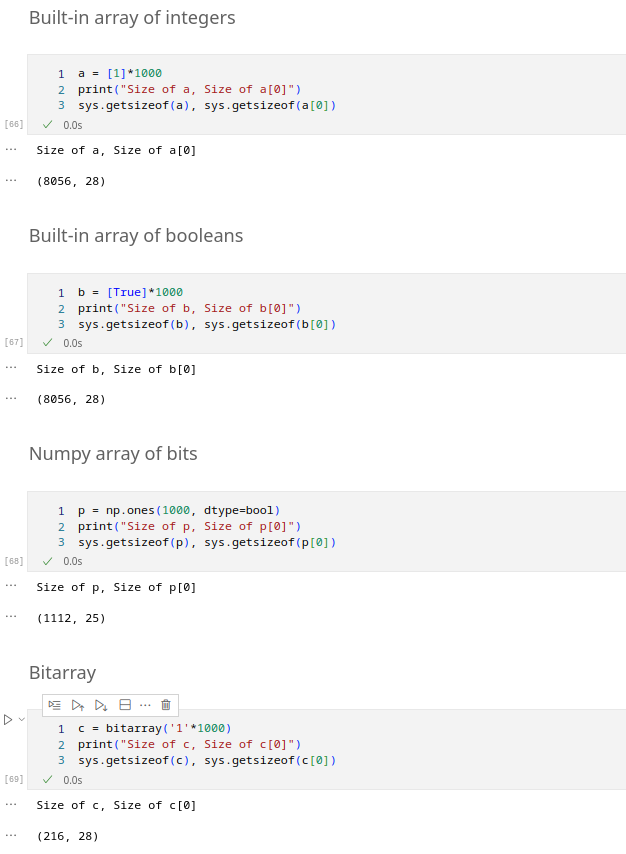
\includegraphics[width=0.6\textwidth]{mem_array.png}
            % \caption{}
            \label{fig:mem_array}
        \end{figure}
\end{frame}

\begin{frame}
        % picture "mem_matrix.png" here
        \begin{figure}
            \centering
            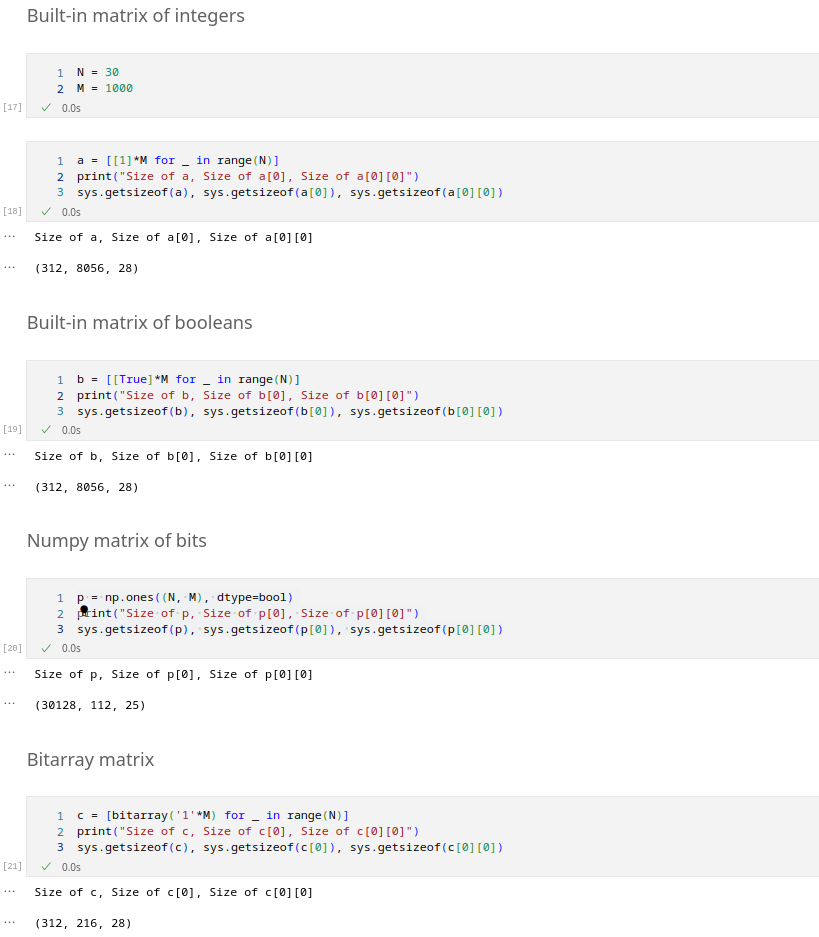
\includegraphics[width=0.55\textwidth]{mem_matrix.png}
            % \caption{}
            \label{fig:mem_matrix}
        \end{figure}
\end{frame}

\begin{frame}
    I tried to profile the code with \texttt{memory-profiler} 
    to find whether the memory occupation
    advantages
    we expect to gain from choosing one data structure over the other
    are actually realized, but I couldn't see any significant difference
    in the memory usage while executing the code, I guess it's because
    the memory required to store the matrices is negligible compared
    to the memory required to store the set of solutions, the set of explored nodes
    and the stack of the recursive calls.
\end{frame}

\section*{Exploring the solutions}

\begin{frame}
    \frametitle{Exploring the solutions}
    Different choices of the cardinality of the domain (columns of the matrix A) and
    the number of sets (rows of the matrix A, rows and columns of the matrix B) 
    lead to different values of:
    \begin{itemize}
        \item the number of solutions found;
        \item the number of explored nodes to find the solutions;
        \item the time required to find the solutions.
    \end{itemize}
    In the following slides I show the values of these quantities for different
    autmatically generated instances of the problem, for time constraints I kept the 
    number of sets in a range between 20 and $\sim400$ and the cardinality of the domain
    in a range between 5 and 14.
\end{frame}

\begin{frame}{Solutions found}
    It's intuitive that the number of solutions found increases
    with the number of sets and decrease with the cardinality of the domain.
    In this case the intuition is confirmed by the solutions found (\ref{fig:sol_5x5}) (at least, those
    found in the chosen dimensions of the problem).
\end{frame}

\begin{frame}
    \begin{figure}
        \centering
        \includegraphics[width=0.6\textwidth]{sol_5x5.pdf}
        % \caption{}
        \label{fig:sol_5x5}
    \end{figure}
\end{frame}

\begin{frame}{Explored nodes}
    It might seem intuitive that, similarly to the previous case, the number of explored nodes
    increases with the number of sets and decreases with the cardinality of the domain,
    however, the same problems that were solved in the previous case display a different
    and less intuitive behaviour in this case (\ref{fig:explored_5x5}).
    The interpretation of this behaviour is that the algorithm has to work harder,
    that is to explore more nodes, to find the solutions for more complex problems, that
    is those problems with a higher number of rows and a higher number of columns.
    Why, fixed the number of rows, a small number of columns implies a higher
    number of explored nodes? I don't know.
\end{frame}

\begin{frame}
    \begin{figure}
        \centering
        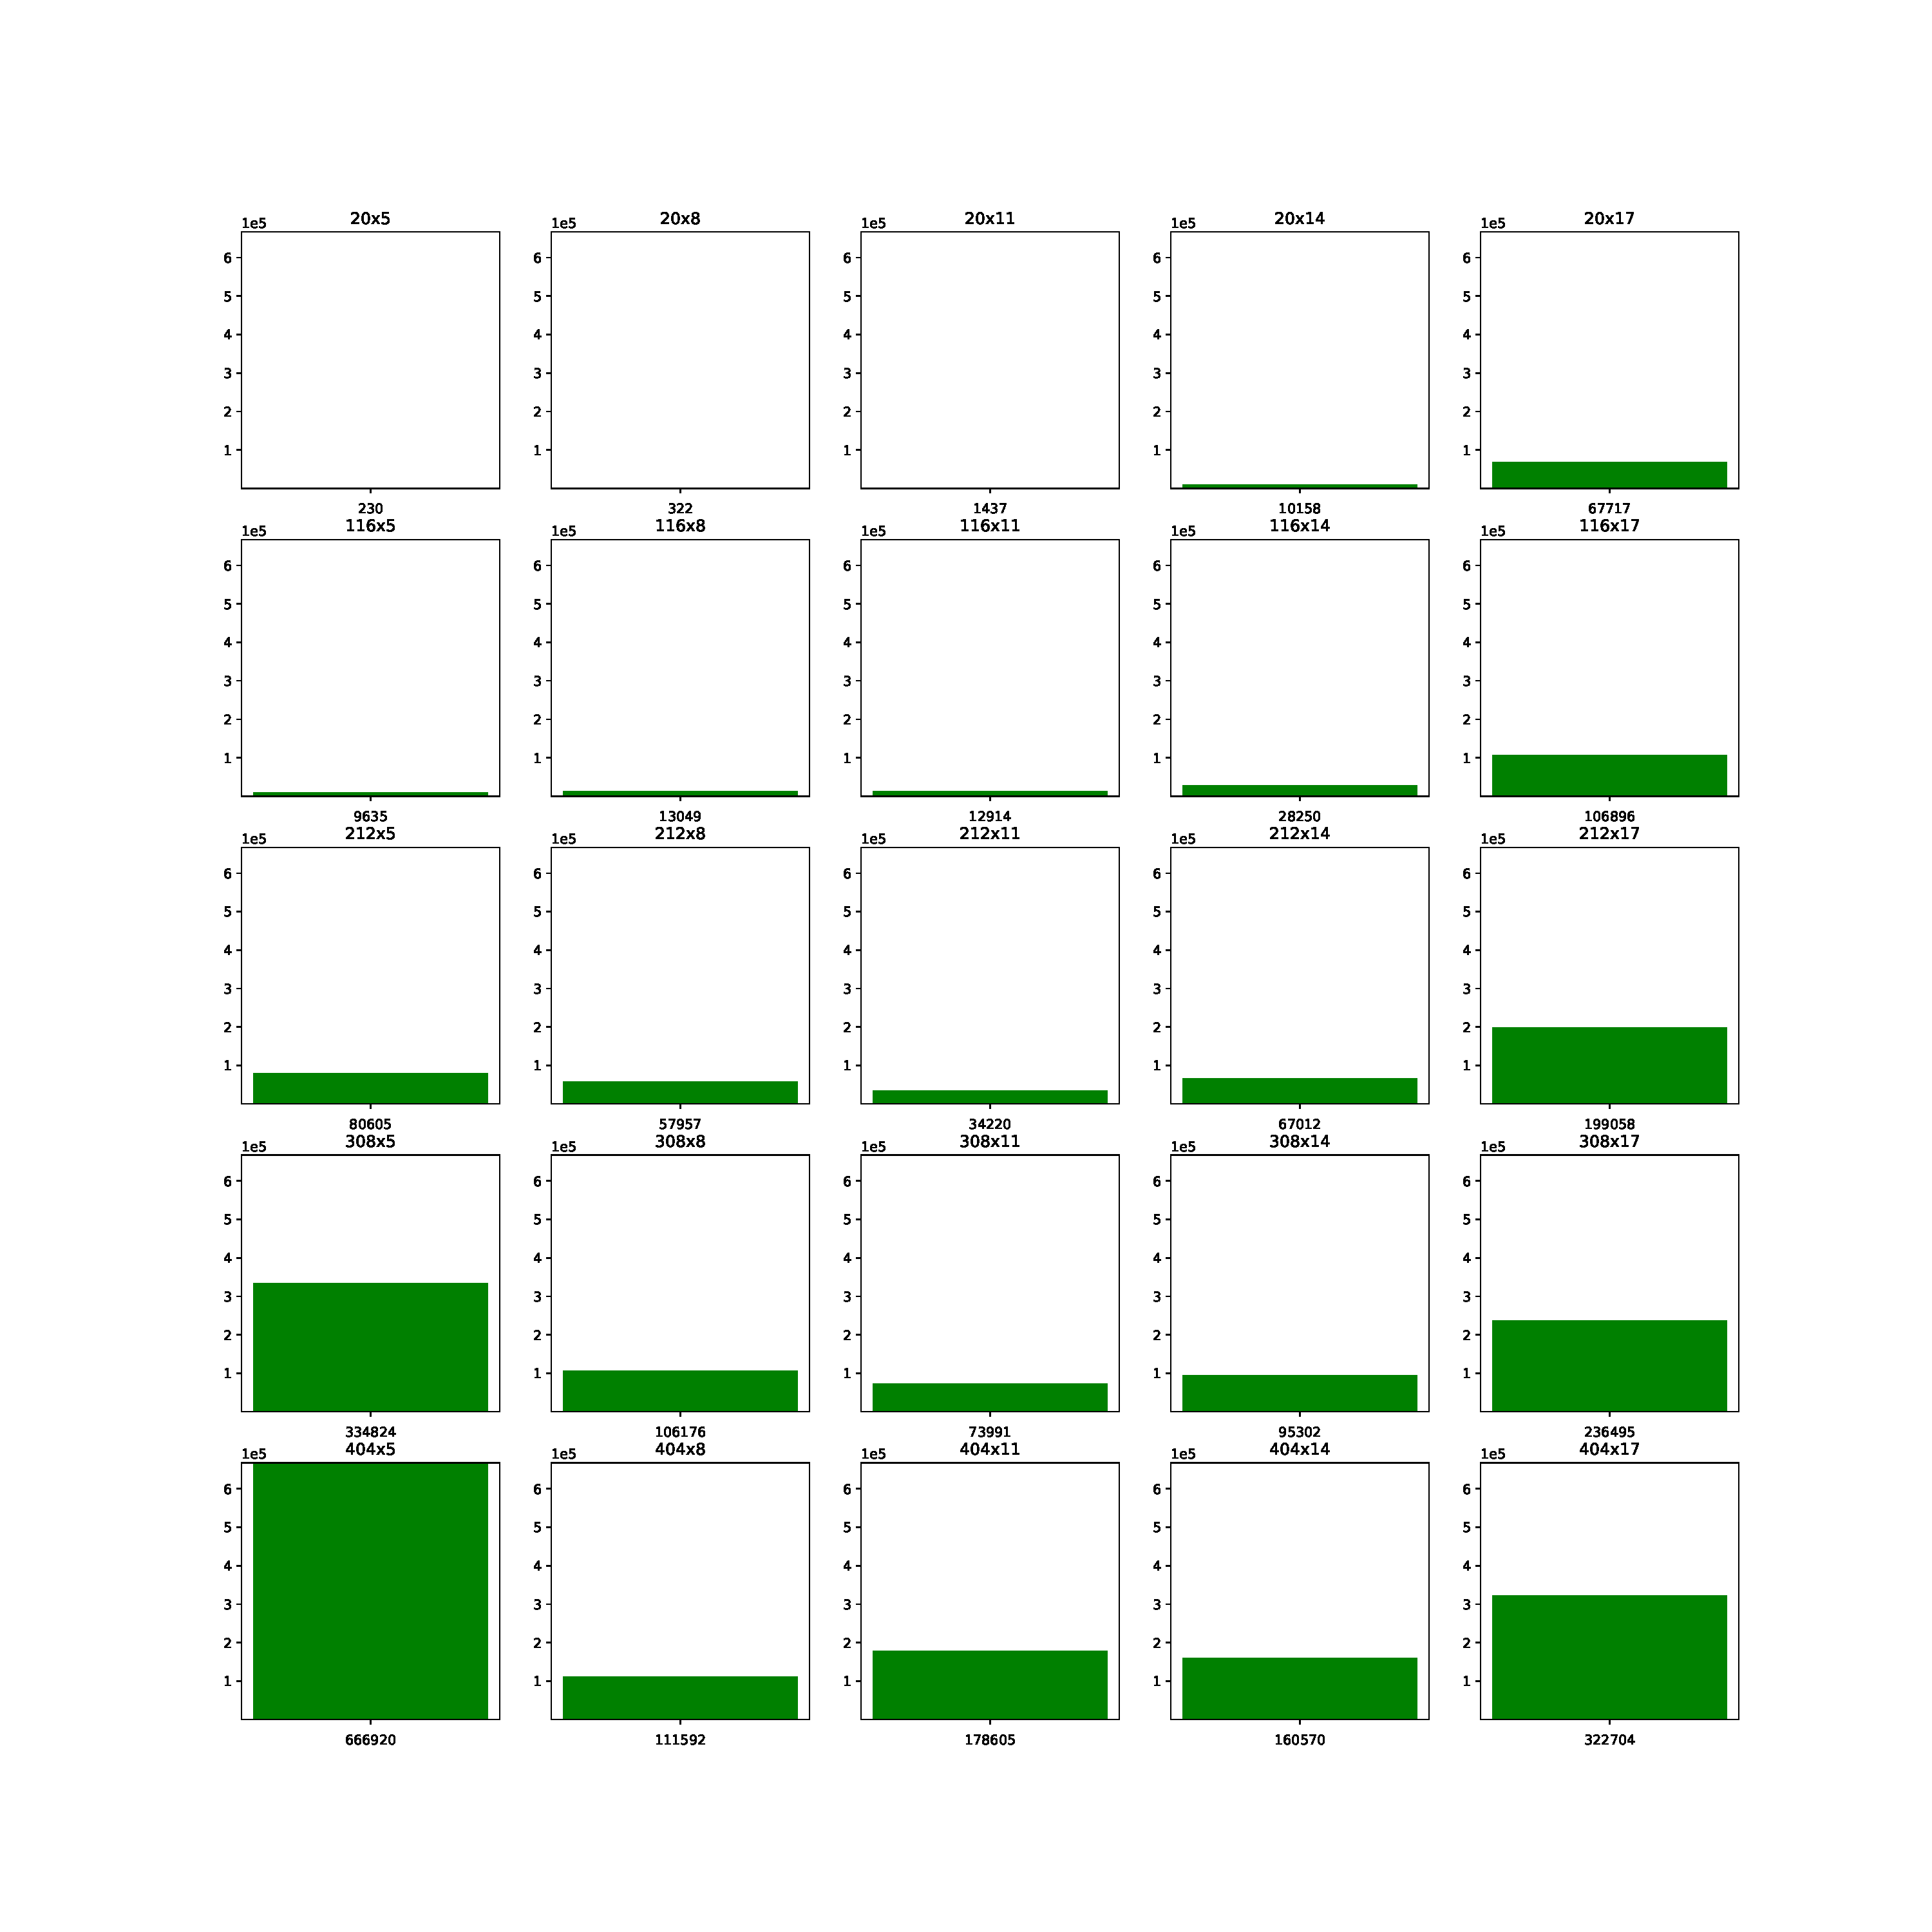
\includegraphics[width=0.6\textwidth]{explored_5x5.pdf}
        % \caption{}
        \label{fig:explored_5x5}
    \end{figure}
\end{frame}

\begin{frame}{Explorable nodes}
    The implemented algorithm chooses to prune the nodes in the tree
    that cannot lead to a plausible solution.
    If the algorithm were to explore all the possible nodes, then for the 
    $i$-th set the number of nodes to explore would be $2^i$,
    hence, if $n$ is the number of sets (rows of A),
    the number of nodes to explore would be $\sum_{i=0}^{n-1} 2^i = 2^n - 1$.

    In figure (\ref{fig:explored_vs_explorable_5x5}) the enormous difference
    between the number of explored nodes and the number of explorable nodes is shown.
    the number of explorable nodes is not exactly $2^n - 1$ because
    the actual computation to represent the explorable nodes is 
    $\sum_{i\in\mathcal{E}}2^i$ where $\mathcal{E}$ is the set of
    explorable  indices
    pointing to rows of A different from an all-zero row (which would be,
    by definition, compatible with any other row).
\end{frame}

\begin{frame}
    \begin{figure}
        \centering
        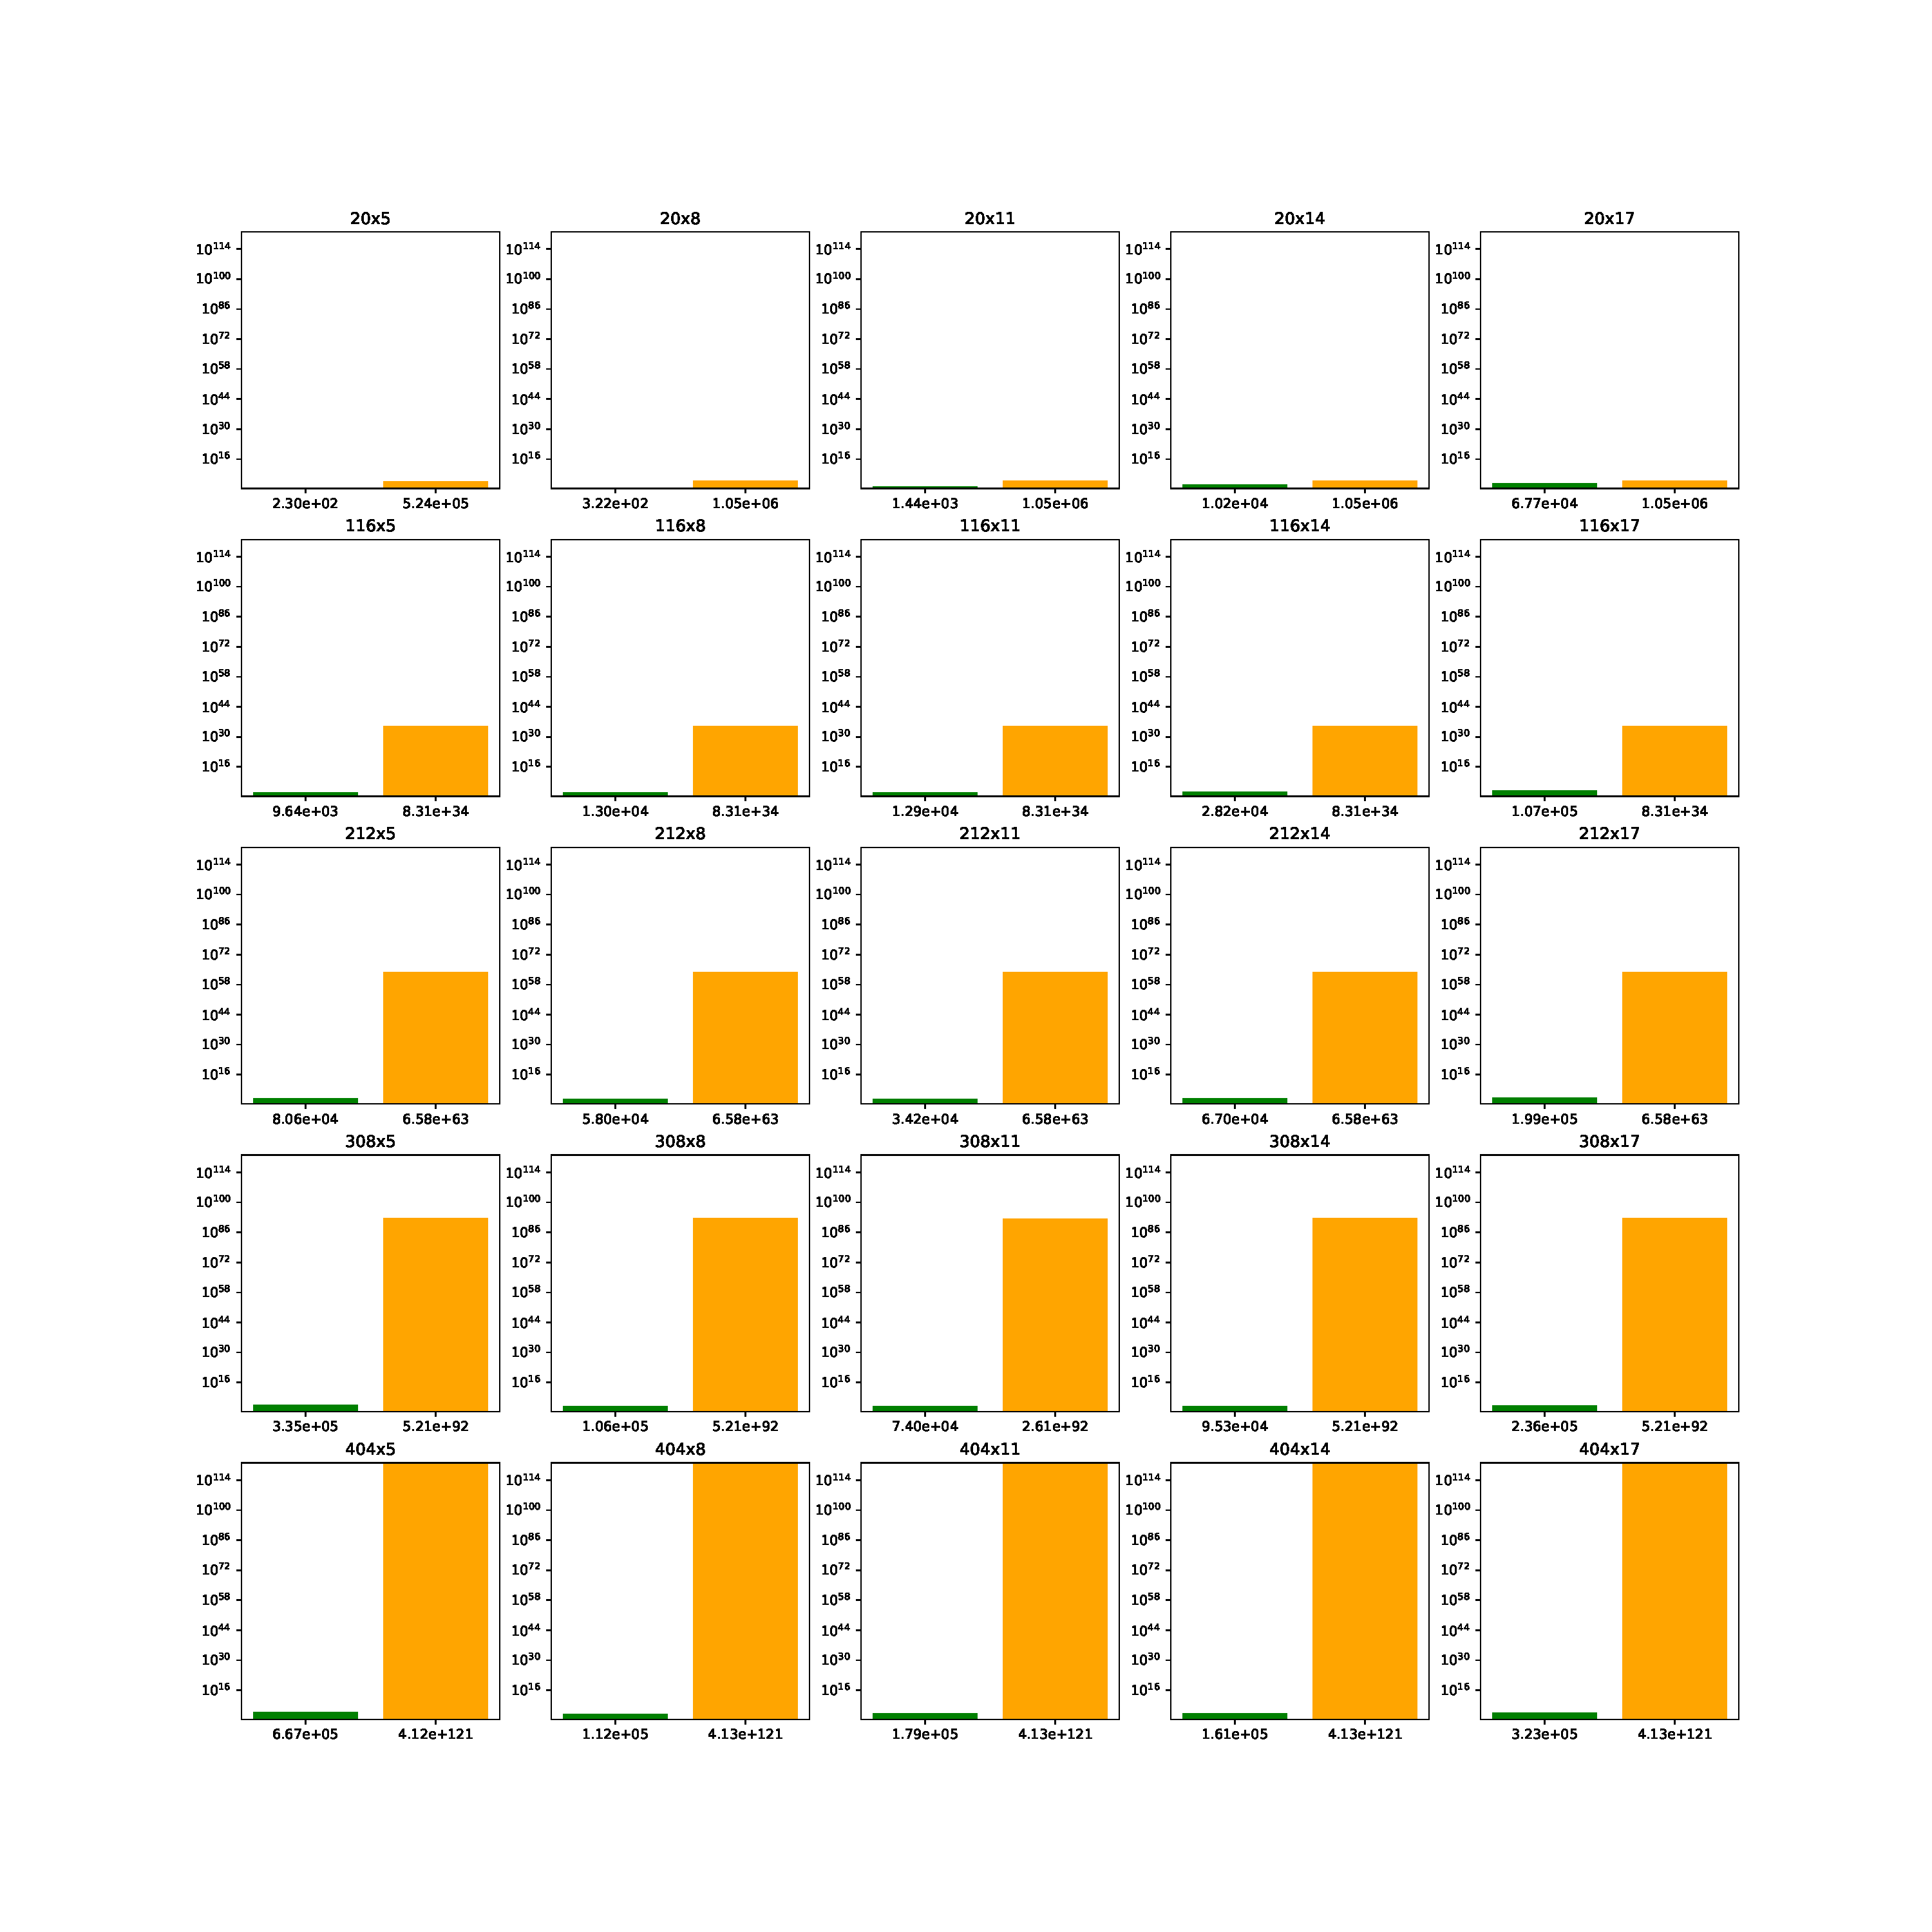
\includegraphics[width=0.6\textwidth]{explored_vs_explorable_5x5.pdf}
        % \caption{}
        \label{fig:explored_vs_explorable_5x5}
    \end{figure}
\end{frame}

\end{document}